\documentclass[preview]{standalone}

\usepackage[english]{babel}
\usepackage{amsmath}
\usepackage{amssymb}

\usepackage[svgnames]{xcolor}
\usepackage{amsthm}\usepackage{amsmath}\usepackage{amsfonts}\usepackage{amssymb}
\usepackage{tikz}
\usetikzlibrary{calc}
\tikzstyle{zero}=[circle,draw=black,fill=white,inner sep=0pt,minimum size=2.5mm]	\tikzstyle{one}=[circle,draw=black,fill=black,inner sep=0pt,minimum size=2.5mm]	\tikzstyle{two}=[circle,draw=black,fill=gray,inner sep=0pt,minimum size=2.5mm] 
\begin{document}

\begin{align*}
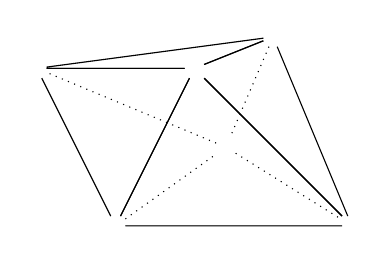
\begin{tikzpicture}[scale=2]	\node (1) at (2,3)  {};	\node [white] (a) at (2.5,3.2) {};	\node (x) at (1,3)  {};	\node (0) at (2.2,2.5)  {};	\node [white] (b) at (1.5,2) {};	\node (z) at (3,2)  {};	\draw (1)-- (a)--(x)--(1);	\draw (1) -- (b)--(x)--(1);	\draw[opacity=0.2](x)--(b);	\draw[dotted](0)--(x);	\draw[opacity=0.2](x)--(a);	\draw[dotted](a) -- (0);   \draw(1)-- (a)--(z)--(1);	\draw(1) -- (b)--(z)--(1);	\draw[opacity=0.2](z)--(b);	\draw [dotted](0)--(z);	\draw [dotted](b) -- (0);\end{tikzpicture}
\end{align*}

\end{document}
